\documentclass{article}
\usepackage{amsfonts, amsmath, amssymb, amsthm, graphicx} % Math 
\graphicspath{ {./images} }
\usepackage{enumitem}

\newtheorem{thm}{Theorem}
\newtheorem{prop}[thm]{Proposition}
\newtheorem{cor}[thm]{Corollary}
\newtheorem{claim}[thm]{Claim}

\newenvironment{problem}[2][Problem]{\begin{trivlist}
\item[\hskip \labelsep {\bfseries #1}\hskip \labelsep {\bfseries #2.}]}{\end{trivlist}}

% title information
\title{Math 158 Textbook Solutions}
\author{Ray Tsai}
\date{1/14/2023}

% main content
\begin{document} 

% placing title information; comment out if using fancyhdr
\maketitle 

% Q1.7.2
\begin{problem}{1.7.2}
    Let $K_{n:r}$ denote the Kneser graph, whose vertex set is the set of
    r-element subsets of an n-element set, and where two vertices form an edge if the
    corresponding sets are disjoint.
    \begin{enumerate}[label=(\alph*)]
    \item Describe $K_{n:1}$ for $n \geq 1$.
    \begin{proof}[Solution]
        Since $\forall v,u \in V(K_{n:1})$, $v \cap u = \emptyset$. Thus, $\forall v,u \in V(K_{n:1})$, $\{v, u\} \in E(K_{n:1})$, which makes $K_{n:1}$ a $K_n$ complete graph.
    \end{proof}
    
    \item Draw $K_{4:2}$ and $K_{5:2}$.
    \begin{proof}[Solution]
        Graphs of $K_{4:2}$ and $K_{5:2}$: \\
        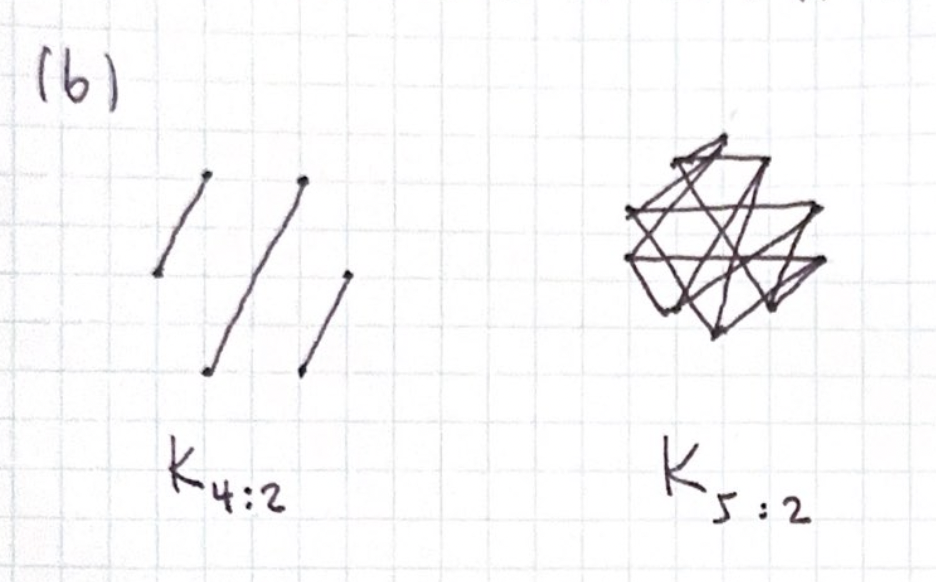
\includegraphics[width=.93\textwidth]{Q172b}
    \end{proof}

    \item Determine $|E({K_{n:r}})|$ for $n \geq 2r \geq 1$.
    
    \begin{proof}[Solution]
        For each $v \in V(K_{n:r}$, $v$ forms edges with other vertices whose vertex set is $r$ of the other $n-r$ elements that are not in the vertex set of $v$, which implies that $d_{K_{n:r}}(v) = {{n-r} \choose {r}}$. Since there are $n \choose r$ vertices in $K_{n:r}$, by the Handshake Theorem, we have  $|E(K_{n:r})| = \binom{n}{r}\binom{n-r}{r}/2$.
    \end{proof}
\end{enumerate}
\end{problem}

% Q1.7.4
\begin{problem}{1.7.4}
    Let $G$ be a digraph such that every vertex has a positive in-degree. Prove that $G$ contains a directed cycle.
\end{problem}
\begin{proof}
    We will prove this by contradiction. Let $v \in V(G)$.  Suppose for the sake of contradiction that $G$ does not contain any directed cycle. Starting from $v$, we can find a path $P$ by tracing back to a vertex with an edge directed to the current vertex we're on. We then add the vertex to $P$ and go to that vertex, and we repeat the previous actions. Since every vertex in $G$ has a positive in-degree, we can always find another vertex that has a directed edge to the current vertex we're on and not in $P$. However, this makes $G$ have infinitely many vertices, which is a contradiction. Therefore, $G$ contains a directed cycle.
\end{proof}

% Q1.7.12
\begin{problem}{1.7.12}
 Let $g$ be an n-vertex graph with $n \geq 2$ and $\delta(G) \geq (n-1)/2$. Prove that $G$ is connected and the diameter of $G$ is at most two.
\end{problem}
\begin{proof}
    We will first prove that $G$ is connected by contradiction. Suppose for the sake of contradiction that $G$ is disconnected. Let $n = |V(G)|$, $v \in V(G)$, $H$ be the component of $G$ that contains $v$. Since $d_G(v) \geq \delta(G) \geq (n-1)/2$, we have $|V(H)| \geq (n-1)/2 + 1 = (n+1)/2$, which implies that other components in $G$ contain at most $n - (n+1)/2 = (n-1)/2$ vertices. However, this shows that $\Delta(G-V(H)) \leq (n-1)/2 - 1 < (n-1)/2$, which contradicts $\delta(G) \geq (n-1)/2$ because $H$ is disconnected to $G-V(H)$. Therefore, $G$ is connected.

    We will now prove that the diameter of $G$ is at most two. Let $u, w \in V(G)$. If $u \in N(w)$, then $d_G(u, w) = 1$. If $u \notin N(w)$, then $N(u), N(w) \in V(G) \backslash \{u, w\}$. Since $|N(u)|, |N(w)| \geq \delta(G) \geq (n-1)/2$, we have $|N(u)| + |N(w)| > n - 2 = |V(G) \backslash \{u, w\}|$. Hence, $|N(u)| \cap |N(w)| \neq \emptyset$, which means that $d_G(u, w) = 2$. Therefore, the diameter of $G$ is at most two.
\end{proof}

% Q1.7.14.a
\begin{problem}{1.7.14.a}
     Let $P$ and $Q$ be the longest paths in a connected graph $G$. Prove that
     \[V(P) \cap V(Q) \neq \emptyset.\]
\end{problem}
\begin{proof}
    We will prove this by contradiction. Let $P, Q$ be the longest paths in a connected graph $G$, with $\{p_1, p_2, \dots, p_{n+1}\}$ and $\{q_1, q_2, \dots, q_{n+1}\}$ as their vertex sets respectively, and $n = |E(P)| = |E(Q)|$.  Suppose for the sake of contradiction that $V(P) \cap V(Q) = \emptyset$. Since $G$ is connected, there must be a path $R$ that starts from $p_i$ and ends at $q_j$, for some $1 \leq i, j \leq n + 1$. Let $m = d_G(p_i, q_j)$. Since $p_i \neq q_j$, we have $m \geq 1$. Let $P'$ be the longer path between $p_1p_2\dots p_i$ and $p_ip_{i+1}\dots p_{n+1}$, $Q'$ be the longer path between $q_1q_2\dots q_j$ and $q_jq_{j+1}\dots q_{n+1}$. By connecting $P'$, $Q'$, and $R$, we get a new path $S$. Since $|E(P')|, |E(Q')| \geq n/2$, $|E(R)| = m \geq 1$, we have $|E(S)| \geq n + 1$, which contradicts that $P, Q$ are the longest paths on $G$.
    Therefore, if $P, Q$ are the longest paths in a connected graph, then $V(P) \cap V(Q) \neq \emptyset$.
\end{proof}

% Q2.5.2
\begin{problem}{2.5.2}
    A tournament is an orientation of a complete graph. Prove that every tournament contains a directed path containing all of its vertices.
\end{problem}
\begin{proof}
    Let $T_n$ be a $n$-vertex tournament. We will prove by induction on $n$ to show that $T_n$ is traceable for all $n$. $T_1$ is obviously traceable as it only contains one vertex. $T_2$ is traceable, as it contains only one directed edge that connects all the vertices in the graph. Suppose that a $T_k$ contains a directed hamiltonian $uv$-path $P$, for some $k \geq 2$. We denote the vertex after $x$ in $P$ as $x^+$, for some $x \in V(P)$. By adding a vertex $w$ and $k$ directed edges to $T_k$, we get a $T_{k+1}$. If $e = (w, u)$ or $(v, w) \in E(T_{k+1})$, we can connect $e$ with $P$ to obtain a hamiltonian path in $T_{k+1}$. If $(w, u), (v, w) \notin E(T_{k+1})$, we know $(u, w), (w, v) \in E(T_{k+1})$ because $N_{T_{k+1}}(w) = V(P)$, which ensures $d_{T_{k+1}}^+(w), d_{T_{k+1}}^-(w) \geq 1$. Hence, there exist $x \in V(P)$ such that $(x, w), (w, x^+) \in E(T_{k+1})$. We can then add $w$ and $(x, w), (w, x^+)$ to $P - (w, w^+)$ to get a directed hamiltonian path in $T_{k+1}$. Thus, if $T_k$ is traceable, then $T_{k+1}$ is also traceable. Therefore, all tournaments are traceable.
\end{proof}

% Q2.5.7
\begin{problem}{2.5.7}
    Prove that a graph $G$ of minimum degree at least $k \geq 2$ containing no triangles contains a cycle of length at least $2k$.
\end{problem}
\begin{proof}
    Let $P$ be the longest path in $G$, say $v_1v_2\dots v_t$. Then $N(v_t) \subseteq V(P)$. Since $G$ does not contain any triangles, if $v_p, v_q \in N(v_t)$ for some $p > q$, then $p - q \geq 2$. Since $|N(v_t)| \geq \delta(G) \geq k$ and $d_P(v_p, v_q) \geq 2$ for some $v_p, v_q \in N(v_t)$, we have $t \geq 2k + 1$ and $v_t$ has a neighbor $v_i$ for some $i \leq t - 2k$, which proves that the cycle $v_i v_{i+1}\dots v_t v_i$ has a length of at least $2k$.
\end{proof}

% Q2.5.9
\begin{problem}{2.5.9}
    The closure of an $n$-vertex graph $G$, denoted $C(G)$, consists in adding edges between any two non-adjacent vertices $u$ and $v$ such that $d_G(u)+d_G(v) \geq n$. Prove that a graph $G$ is hamiltonian if and only if $C(G)$ is hamiltonian.
\end{problem}
\begin{proof}
    If $G$ is hamiltonian, $G$ contains a hamiltonian cycle $H \subseteq G$. Since $C(G)$ contains $G$ and $V(C(G)) = V(G)$, we have $H \subseteq G \subseteq C(G)$, and thus $C(G)$ is hamiltonian. 
    
    Suppose that $C(G)$ has a hamiltonian cycle $F$. If $F$ does not contain any edges that are not in $G$, then $G$ is hamiltonian. Otherwise, there exists $\{u, v\} \in E(F)$ such that $\{u, v\} \notin E(G)$, which implies $d_G(u)+d_G(v) \geq n$. Let $P = F - \{u, v\}$ be a hamiltonian $uv$-path of $C(G)$, say $v_1v_2\dots v_n$, and $N(v)^+ = \{v_{i+1} : v_i \in N_G(v)\}$. We then have $N(v)^+ \cup N(u) \subseteq V(P)\backslash \{u\}$, which shows that $|N(v)^+ \cup N(u)| \leq n - 1$. Since $|N(v)^+| + |N(u)| = d_G(u)+d_G(v) \geq n$, we have
    \begin{align}
        |N(v)^+ \cap N(u)|
        &= |N(v)^+| + |N(u)| - |N(v)^+ \cup N(u)| \\
        &\geq n - (n - 1) = 1.
    \end{align}
    Hence, $N(v)^+ \cap N(u) \neq \emptyset$. Let $v_k \in N(v)^+ \cap N(u)$, we can then get a new hamiltonian cycle $P - \{v_k, v_{k+1}\} + \{u, v_{k+1}\} + \{v_k, v\}$. This shows that all $e \in E(F)\backslash E(G)$ can be removed from $F$ to obtain a hamiltonian cycle that only consists of edges in $G$, which shows that $G$ is hamiltonian. Therefore, $C(G)$ is hamiltonian if and only if $G$ is hamiltonian.
\end{proof}

%2.5.11
\begin{problem}{2.5.11}
    Let $G$ be a hamiltonian bipartite graph of a minimum degree of at least three. Prove that $G$ contains at least two hamiltonian cycles.
\end{problem}
\begin{proof}
    Let $C$ be a hamiltonian cycle in bipartite graph $G(A,B)$, and let $u, v, w \in A$ such that $N_C(u) = \{v, w\}$. Consider the hamiltonian $uv$-path $P = C - \{u, v\}$. Since $G$ is bipartite and $v \in B$, we know $N(v)^+ \in B$, and thus the vertices of $P$ obtained by all possible rotations are all in $B$. Let $G'(A', B') \subseteq G$ such that $C \subseteq G'$ and $d_{G'}(b) = 3$ for all $b \in B'$. We know $G'$ exists because $\delta(G) \geq 3$. Let $H$ be a graph whose vertices are hamiltonian paths of $G'$ starting with the edge $\{u, w\}$, where two hamiltonian paths in $G'$ form an edge of $H$ if they are obtained from one another by rotation. If $Q \in H$ is a hamiltonian path that ends at a vertex $x$, then $Q$ has $3 - 1 = 2$ possible rotations in $G'$ unless $\{u, x\} \in E(G')$, in which case would have $3 - 2 = 1$ rotations instead. In the latter case, $Q$ together with $\{u, w\}$ would form a hamiltonian cycle in $G'$. By the Handshake Theorem, since the number of vertices with odd degrees is even, there is an even number of paths $Q$ in $G'$ which ends at a neighbor of $u$. Therefore, $G'$ has an even amount of hamiltonian cycles containing $\{u, w\}$. Since $G'$ already contains a hamiltonian cycle $C$, it must contain some other hamiltonian cycle $C'$. Since $C, C' \subseteq G' \subseteq G$, $G$ has at least two hamiltonian cycles.
\end{proof}

% 3.8.1
\begin{problem}{3.8.1}
    A school with $20$ professors forms $10$ committees, each containing $6$ professors, such that every professor is on exactly $3$ committees. Prove that it is possible to select a distinct representative from each committee.
\end{problem}

\begin{proof}
    Let $G$ be a bipartite graph with the set of all professors and committees, where each professor and committee form an edge if the professor is in the committee. Let $C$ be a subset of the set of all committees. Since each committee has an edge with $6$ professors, we know that $C$ is incident to $6|C|$ edges. Since each professor has an edge with $3$ committees, we know that $N(C)$ is incident to $3|N(C)|$ edges. Since the edges $N(C)$ is incident to include the edges $C$ is incident to, $3|N(C)| \geq 6|C|$, and thus $|N(C)| \geq |C|$. By Hall's Theorem, there is a matching saturating the set of all committees, so it is possible to select a distinct representative from each committee.
\end{proof}

% 3.8.2
\begin{problem}{3.8.2}
    A tiling of an $m \times n$ chess board is a set of dominoes that cover all the squares on the chess board exactly once (each domino covers two adjacent squares).
\end{problem}
\begin{enumerate}[label=(\alph*)]
    \item For which $m \geq 1$ and $n \geq 1$ does an $m \times n$ chess board having a tiling?
    \begin{proof}[Solution]
        Since the number of squares on the chess board must be even to have a perfect matching, $m$ or $n$ is even. Assume, without loss of generality, that $m$ is even. We will prove by induction on $m$. If $m = 2$,  then we can match each square in one column to one in the adjacent column that is adjacent to it, and this is a perfect matching $M_2$. Suppose that there is a perfect matching $M_k$ for each $k \times n$ chessboard, where $2 \leq k \leq m$ and is even. We can then split a $(m + 2) \times n$ chessboard into a $2 \times n$ and $m \times n$ board. We can then find a perfect matching $M_2 \cup M_m$. This also shows true for even $n$. Therefore, for all $(m,n) \in \{(a, b) \in \mathbb{N}^2: ab \text{ is even}\}$, an $m \times n$ chessboard has tiling. 
    \end{proof}
    
    \item If we remove two squares from an $m \times n$ chessboard, when do the remaining squares have a tiling?
    \begin{proof}[Solution]
        There must be an even amount of squares to have tiling, so if a $m \times n$ chessboard has tiling after two squares removed, then the $m \times n$ chessboard also has an even amount of squares. Thus, $m$ or $n$ needs to be even.

        Assume, without loss of generality, that $m$ is even. Let $G$ be a grid graph whose vertex set contains all squares on a $m \times n$ chessboard, and each pair of vertices forms an edge if they are adjacent to each other on the board. Since $m$ is even, $G$ has a perfect matching. Let $v_{xy}$ correspond to the square in the $x$th row and $y$th column, for some $1 \leq x \leq n$, $1 \leq y \leq m$. Let $\{c_1, c_2\}$ be a set of two colors. We color $v_{xy}$ with $c_1$ if $x + y$ is even and $c_2$ if $x + y$ is odd. This shows that every square can be colored with no same-colored squares being adjacent. Since each domino covers a $c_1$ square and a $c_2$ square, each color must have the same number of squares to have tiling. Therefore, if we remove two squares with the same color, then $G$ does not have a tiling.
        
        Suppose that we remove two squares $u, v$ with different colors. If $n = 1$, then $G - \{u\} - \{v\}$ has a tiling if there are only even components.
        \begin{claim}
            If $m = 2$, then $G - \{u\} - \{v\}$ has a tiling.
        \end{claim}
            Suppose that $u, v$ are each in the first and last rows and $n$ is some natural number. Consider the case where $n$ is odd. Since $u, v$ have different colors, $u, v$ are in different columns. This means that the two columns in $G - \{u\} - \{v\}$ both have $n - 1$ number of squares, which is even. Consider the case where $n$ is even. Since $u, v$ has different colors, $u, v$ are in the same column. This means that the two columns in $G - \{u\} - \{v\}$ have $n$ and $n - 2$ numbers of squares respectively, which are also even. Thus, in both cases, we can tile along the columns and cover all squares, which is a tiling. Suppose that $u, v$ are in the $i$th and $j$th rows, for some $1 < i \leq j < n$. We can then remove the first $i - 1$ rows and the last $n - j$ rows, as there are two columns so we can find a tiling of them by putting a domino in each row. What is left is a $2 \times (j - i + 1)$ board with two corners on both sides removed, which we just proved to have tiling in the first case. Therefore, $G - \{u\} - \{v\}$ has a tiling if $m = 2$.
            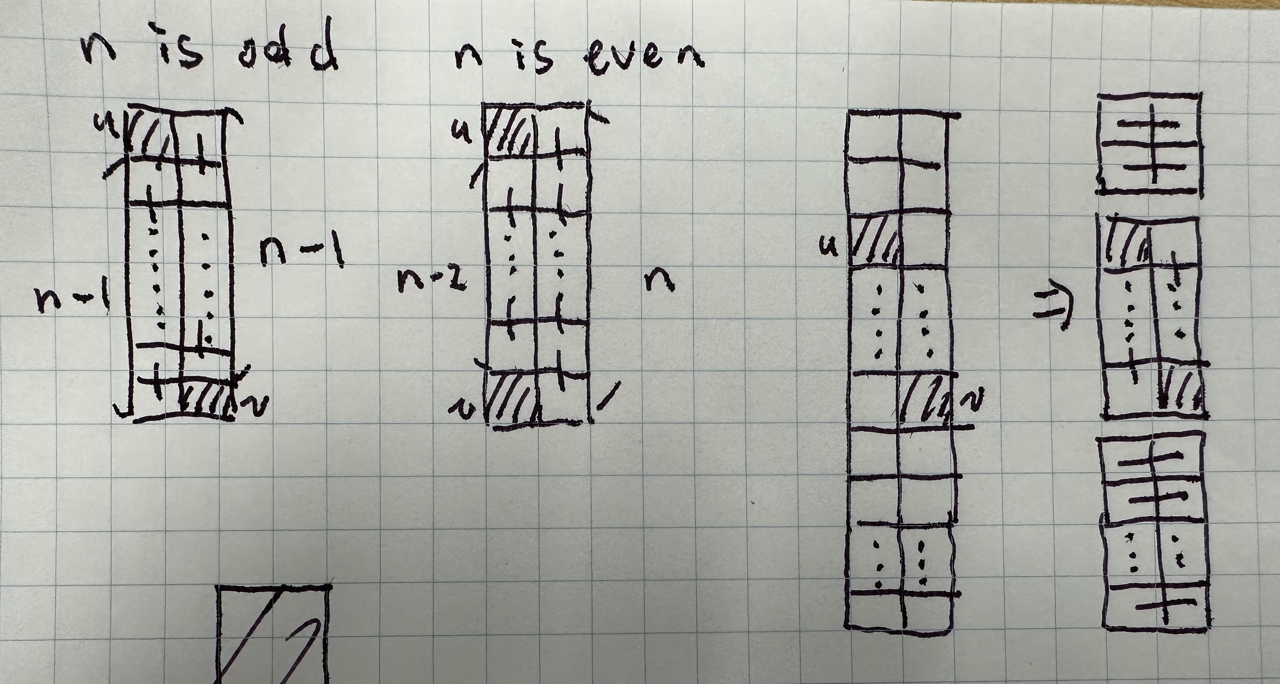
\includegraphics[width=.93\textwidth]{Q382b1}
        \begin{claim}
            Suppose that $n \geq 2$. If $u, v$ are each in a $2 \times 2$ corner on the opposite side, then $G - \{u\} - \{v\}$ has a perfect matching.
        \end{claim}
        Assume, without loss of generality, that $u$ is in the top left $2 \times 2$ corner and $v$ is in the bottom right $2 \times 2$ corner. Since the $(m - 2) \times (n - 2)$ squares on the bottom left have a perfect matching $M_1$, as it has an even side, we can first take it out. What is left are the first two rows and last two columns of $G$, so we can split it into two parts, a $(m - 2) \times 2$ board $A$ that contains $u$ and a $(2 \times n)$ board $B$ that contains $v$. Let $w \in V(B) \cap N_G(V(A))$ such that $w$ shares the same color with $u$. We remove $w$ from $B$ to $A$, and we then have two parts, $A + \{w\}$ and $B - \{w\}$. We can view $A + \{w\}$ as a $2 \times (m - 1)$ board missing two different color squares $u$ and a square next to $w$. By Claim 1, since both $A + \{w\}$ and $B - \{w\}$ have exactly two columns and are missing two different-colored squares, $A + \{w\}$ and $B - \{w\}$ each has a perfect matching $M_2$ and $M_3$ respectively. Therefore, $G - \{u\} - \{v\}$ has a perfect matching $M_1 \cup M_2 \cup M_3$.

        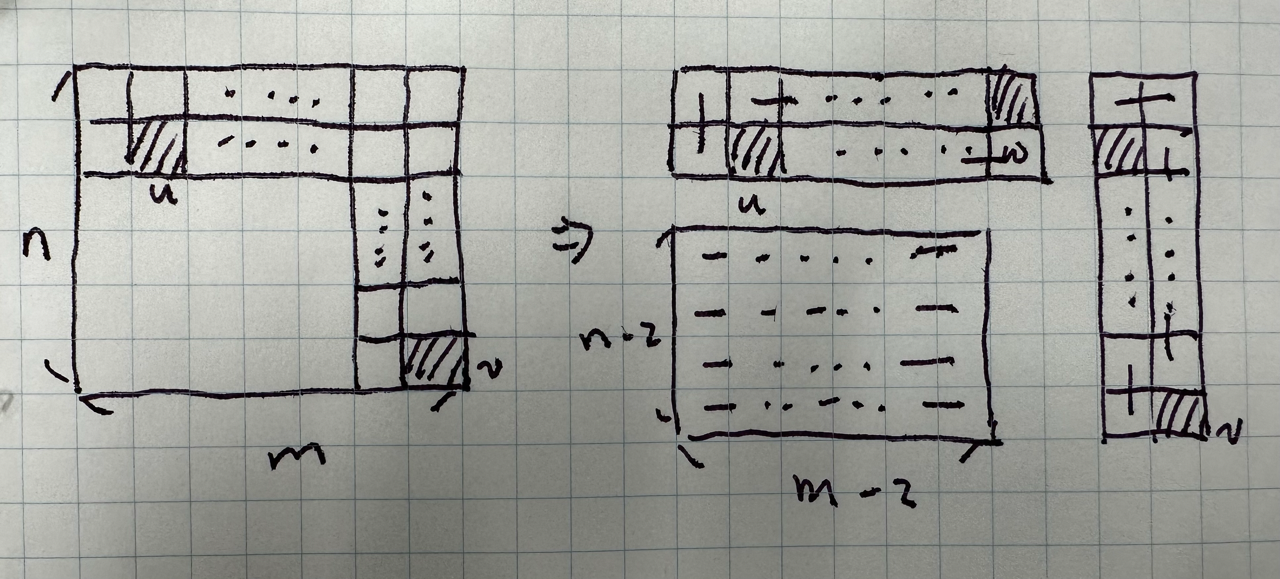
\includegraphics[width=.93\textwidth]{Q382b2}

        Finally, we will show that $G - \{u\} - \{v\}$ has a perfect matching for all $m, n \geq 2$, $m$ is even. Suppose that $u$ is in the $i$th row $j$th column and $v$ is in the $k$th row $l$th column of $G$. Assume, without loss of generality, that $k \geq i$ and $l \geq j$. We can first take out a $m \times (i - 1)$ board $I$ that contains the first $(i - 1)$ rows of $G$ and a $m \times (n - k)$ board $K$ that contains the last $(n - k)$ rows of $G$. Since they both have an even side $m$, they have a perfect matching $M_i$ and $M_k$ respectively. What's left is a $m \times (k - i + 1)$ board $G'$. We can then take out the left-most $2\alpha$ and right-most $2\beta$ columns of $G'$, where $\alpha$ is the greatest integer such that $2\alpha < j$ and $\beta$ is the greatest integer such that $m - 2\beta > l$ and obtain a $2\alpha \times (k - i + 1)$ board $J$ and a $2\beta \times (k - i + 1)$ board $L$. Since $J$ and $L$ each have an even side $2\alpha$ and $2\beta$, they have perfect matching $M_J$ and $M_L$ respectively. What is left is a $(m - 2(\alpha + \beta)) \times (k - i + 1)$ board $C$ with $u, v$ in opposite side $2 \times 2$ corners. By Claim 2, $C$ contains a perfect matching $M_C$. We now found a perfect matching $M_I \cup M_J \cup M_K \cup M_L \cup M_C$ of $G - \{u\} - \{v\}$. Therefore, if we remove two squares from a $m \times n$ chessboard, it has tiling if and only if $mn$ is even and the two removed squares have different colors and all boards have an even number of squares.
        
        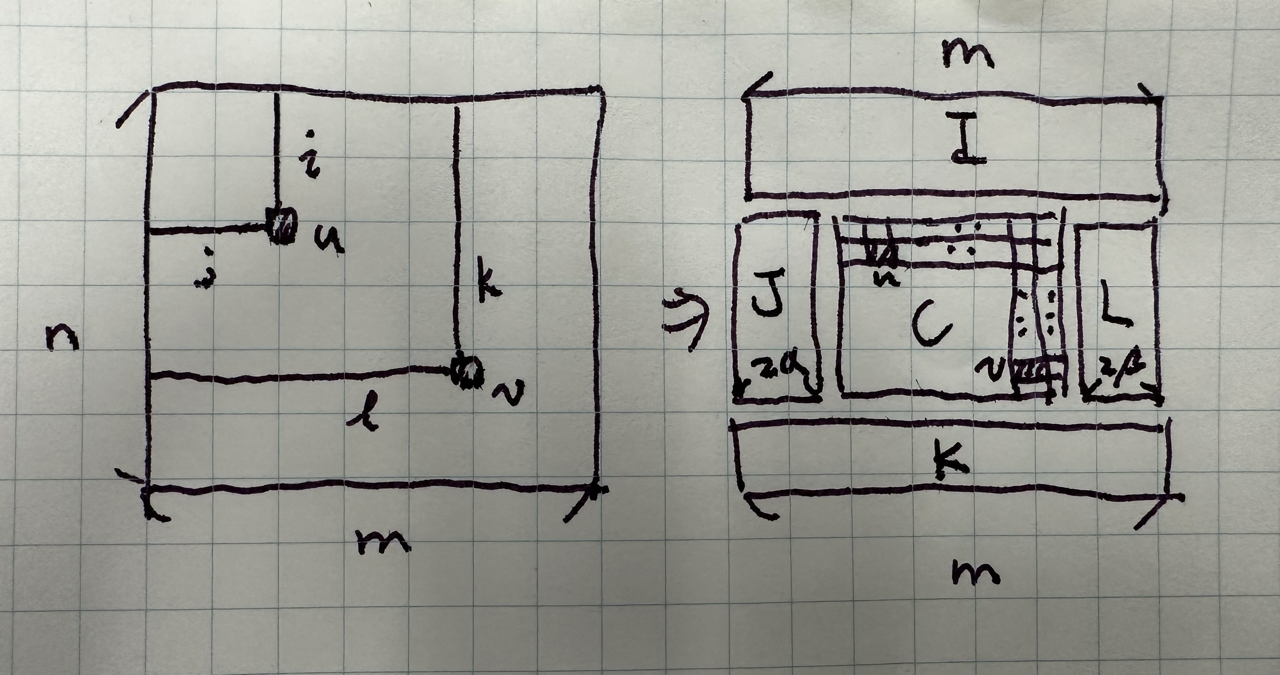
\includegraphics[width=.93\textwidth]{Q382b3}
    \end{proof}
\end{enumerate}

% 3.8.3
\begin{problem}{3.8.3}
    Let $e$ be an edge of a connected cubic graph such that $G - e$ is disconnected. Prove that every perfect matching of $G$ contains $e$.
\end{problem}

\begin{proof}
    Suppose for sake of contradiction that there exists a perfect matching $M$ of $G$ such that $e \notin M$. Let $G_1$ and $G_2$ be the two components in $G - e$ respectively. Since $e \notin M$, $G - e$ has a perfect matching, and thus $G_1$ and $G_2$ both have a perfect matching. Since each vertex in $G$ is degree three and we only removed one edge, $G_1$ and $G_2$ each have an even number of vertices with degree $3$ and a single vertex with degree $2$. This makes $G_1$ and $G_2$ odd components, which contradicts that they both have a perfect matching. Therefore, $e$ must be in the perfect matching of $G$.
\end{proof}

% 3.8.5
\begin{problem}{3.8.5}
    Determine $\chi{'}(G)$ when $G$ is the Petersen graph.
\end{problem}

\begin{proof}
    Since the maximum degree of the Petersen graph is $3$, its edge chromatic number is $3$ or $4$ by Vizing's Theorem. Suppose the Petersen graph can be $3$ edge colored with $\{1, 2, 3\}$. Since Petersen's graph is cubic, each vertex is incident with edges of all colors. Take an edge $\{u, v\}$ on the pentagon and color it with $1$. Let $x$ be $u$'s neighbor on the pentagram and $y$ be that of $v$'s. Since $\{u, x\}$ and $\{v, y\}$ cannot be colored with $1$, there are $2$ edges with color $1$ on the pentagram. Since a pentagon cannot be $2$ edge-colored, at least three colors appear on the edges of the pentagon. This means that all three colors appear at least twice on the $5$ edges of the pentagram, contradiction. Therefore, the edge chromatic number of the Petersen graph is $4$. 
\end{proof}

% 3.8.8
\begin{problem}{3.8.8}
    
\end{problem}
\begin{enumerate}[label=(\alph*)]
    \item Let $G$ be an $n$ by $n$ bipartite graph of minimum degree more than $n/2$. Prove that $G$ has a perfect matching.
    \begin{proof}[Solution]
        Suppose that there is a non-hamiltonian $n$ by $n$ bipartite graph of minimum degree at least $n /2$. Amongst all such graphs, let $H(A, B)$ be one with parts $A$ and $B$ and a maximum number of edges. If we add an edge $e = \{v_1, v_{2n}\}$ between non-adjacent vertices in $H$, we would have a graph with a hamiltonian cycle $C$, and so $C - e$ is a hamiltonian path in $H$, say $v_1v_2 \dots v_{2n}$. Assume, without loss of generality, that $v_1 \in A$ and $v_{2n} \in B$. Let $N(v_1)^+ = \{v_{i+1} : v_i \in N(v_1)\}$. Since $N(v_1)^+ \cup N(v_{2n}) \subseteq A$, we have $|N(v_1)^+ \cup N(v_{2n})| \leq n$. Since $\delta(H) > n/2$, we have $|N(v_1)^+| + |N(v_{2n})| \geq n + 1$. Thus, we have
        \begin{align}
            |N(v_1)^+ \cap N(v_{2n})| 
            &= |N(v_1)^+| + |N(v_{2n})| - |N(v_1)^+ \cup N(v_{2n})| \\
            &\geq n + 1 - n = 1.
        \end{align}
        This shows that $N(v_1)^+ \cap N(v_{2n}) \neq \emptyset$, which proves that $H$ contains a hamiltonian cycle, a contradiction. Therefore, there exists a hamiltonian path $P$ in $G$ such, say $u_1 u_2 \dots u_{2n}$. Let $f = \{(u_i, u_{i+1}) : i \text{ is even}\}$. We can then find a perfect matching $M = P - f$ of $G$. Hence, $G$ has a perfect matching.
    \end{proof}
    
    \item Let $G$ be a $2n$-vertex graph of minimum degree at least $n$. Prove that $G$ has a perfect matching.

    \begin{proof}[Solution]
        If $n = 1$, $G$ itself is a perfect matching for $G$. Suppose that $n \geq 2$. By Dirac's Theorem, since $\delta(G) \geq |V(G)|/2$, $G$ contains a hamiltonian path $P$, say $v_1v_2 \dots v_{2n}$. Let $e = \{(v_i, v_{i+1}) \in E(P) : i \text{ is even}\}$, then $M = P - e$ is a perfect matching in $G$. Therefore, $G$ has a perfect matching.
    \end{proof}
\end{enumerate}

% 3.8.9
\begin{problem}{3.8.9}
    Let $A_k$ be the set of subsets of $\{1,2, \dots , n\}$ of size $k$. Prove that for $k < n/2$, there is an injective function $f: A_k \rightarrow A_{k+1}$ such that $a \subseteq f(a)$ for all $a \in A_k$. For instance, if $k = 1$ and $n = 3$ then the function
    \[
        f(\{1\}) = \{1, 2\} \quad f(\{2\}) = \{2, 3\} \quad f(\{3\}) = \{1, 3\}
    \]
    is an example of such a function $f: A_1 \rightarrow A_2$.
\end{problem}

\begin{proof}
    Let $G$ be a bipartite graph with parts $A_k$ and $A_{k+1}$, for some $k < n / 2$, and each $a_k \in A_k$ forms an edge with $a_{k+1} \in A_{k+1}$ if $a_k \subset a_{k+1}$. Since $k < n / 2$, $|A_k| = {n \choose k} \leq {n \choose k + 1} = |A_{k+1}|$. For each $a_k \in A_k$, there are $n - k$ number of $a_{k+1} \in A_{k+1}$ such that $a_k \subset a_{k+1}$, so each $a_k$ has $n - k$ neighbors. For each $a_{k+1} \in A_{k+1}$, there are $k + 1$ number of $a_k \in A_k$ such that $a_k \subset a_{k+1}$, so each $a_{k+1}$ has $k + 1$ neighbors. Since both sides are incident to the same number of edges, we know $(n - k)|A_k| = (k + 1)|A_{k+1}|$, and so $n - k \geq k + 1$ because $|A_k| \leq |A_{k+1}|$. Let $S \subseteq A_k$. We know there are $(n - k)|S|$ edges that are incident with $S$, and there are $(k + 1)|N(S)|$ edges that are incident with $N(S)$. Since the edges that are incident with $N(S)$ contain the ones that are incident with $S$, we have $(k + 1)|N(S)| \geq (n - k)|S| \geq (k + 1)|S|$, and so $|N(S)| \geq |S|$. Therefore, by Hall's Theorem, there is a matching saturating $A_k$ in $G$, which shows that there is an injection from $A_k$ to $A_{k+1}$.
\end{proof}

% 3.8.11
\begin{problem}{3.8.11}
    Let $A$ be an $n$ by $n$ matrix of zeros and ones. Suppose every row and every column of $A$ has exactly $k$ ones. Prove that we can pick $n$ ones from $A$, no two in the same row or column.
\end{problem}

\begin{proof}
    Let $G$ be a $n$ by $n$ bipartite graph with the set of rows $R$ and columns $C$ of $A$ as its two parts, where $r \in R$ and $c \in C$ form an edge if the $r$th row $c$th column of $A$ is one. We know that $G$ is $k$-regular. Let $S \subseteq R$. We know that $S$ is incident to $k|S|$ edges and $N(S)$ is incident to $k|N(S)|$ edges. Since the edges $N(S)$ is incident to include the edges $S$ is incident to, $k|N(S)| \geq k|S|$, and thus $|N(S)| \geq |S|$, Hall's condition met. Therefore, there exists a perfect matching of $G$, and thus we can pick $n$ ones from $A$ such that no two are in the same row or column.
\end{proof}

% 3.8.17
\begin{problem}{3.8.17}
    An independent set in a graph G is a set $X \subseteq V (G)$ such that $e(X) = 0$, and the independence number $\alpha(G)$ is the largest size of an independent set in $G$. A vertex cover of $G$ is a set of vertices $X \subset V(G)$ such that $e \cap X \neq \emptyset$ for every edge $e \in E(G)$. The minimum size of a vertex cover of $G$, the vertex cover number, is denoted $\beta(G)$.
\end{problem}

\begin{enumerate}[label=(\alph*)]
    \item Prove that for any graph $G$, $\alpha(G) + \beta(G) = |V(G)|$.

    \begin{proof}
        Let $C$ be the smallest vertex cover of $G$, and let $I$ be the largest independent set in $G$. First, Suppose for the sake of contradiction that $|C \cup I| < |V(G)|$. Let $L = V(G) \backslash (C \cup I) \neq \emptyset$. Since there does not exist $e \in E(G)$ such that $e \subseteq V(G) \backslash C$, we know $e(L) = 0$, and thus $e(L \cup I) = 0$, which makes $L \cup I$ a larger independent set, contradiction. Therefore, $|C \cup I| = |V(G)|$. Suppose for the sake of contradiction that $C \cap I \neq \emptyset$. Let $v \in C \cap I$. Since $v \in I$, we know $N(v) \subseteq V(G) \backslash I \subseteq C$. Since all neighbors of $v$ are in $C$, we can remove $v$ to get a smaller vertex cover $C \backslash \{v\}$, contradiction. Therefore, $C \cap I = \emptyset$, and thus $|V(G)| = |I \cup C| = |I| + |C| = \alpha(G) + \beta(G)$.
    \end{proof}

    \item  Prove that $\mu(G) \leq \beta(G) \leq 2\mu(G)$.
    
    \begin{proof}
        Let $M$ be the maximum matching of $G$, and $C$ be the minimum vertex cover. Since no two exposed vertices form an edge, the neighbors of exposed vertices are all saturated vertices, so the set of all saturated vertices is a vertex cover. Thus, $\beta(G) \leq 2\mu(G)$. For each edge $e \in M$, we know $e \cap C \neq \emptyset$, so $\mu(G) \leq \beta(G)$. Therefore, $\mu(G) \leq \beta(G) \leq 2\mu(G)$.
    \end{proof}
\end{enumerate}

% 4.7.2
\begin{problem}{4.7.2}
    Determine $\chi{'}(G)$ and $\chi(G)$ for each of the graphs shown below.
    
    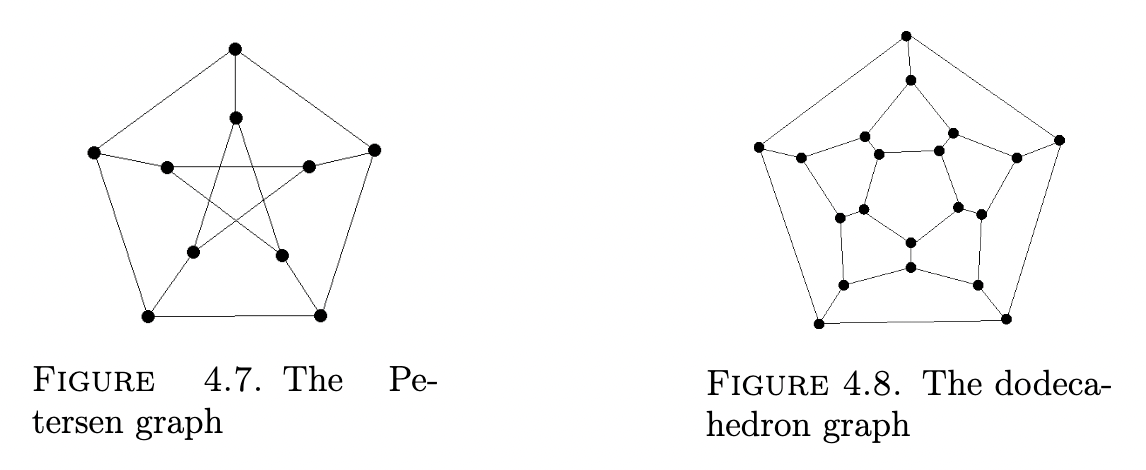
\includegraphics[width=.93\textwidth]{Q472}
\end{problem}

\begin{proof}
    Since the maximum degree of the Petersen graph is $3$, its edge chromatic number is $3$ or $4$ by Vizing's Theorem. Suppose the Petersen graph can be $3$ edge colored with $\{1, 2, 3\}$. Since Petersen's graph is cubic, each vertex is incident with edges of all colors. Take an edge $\{u, v\}$ on the pentagon and color it with $1$. Let $x$ be $u$'s neighbor on the pentagram and $y$ be that of $v$'s. Since $\{u, x\}$ and $\{v, y\}$ cannot be colored with $1$, there are $2$ edges with color $1$ on the pentagram. Since a pentagon cannot be $2$ edge-colored, at least three colors appear on the edges of the pentagon. This means that all three colors appear at least twice on the $5$ edges of the pentagram, contradiction. Therefore, the edge chromatic number of the Petersen graph is $4$. 

    Since the Petersen graph contains an odd cycle, it cannot be $2$-colored. By Brook's Theorem, since the Petersen graph is not a complete graph nor an odd cycle, it can be $3$-colored because the maximum degree is $3$.

    Let $D$ be a dodecahedron graph. Since $D$ contains an odd cycle, $\chi{'}(D), \chi(D) \geq 3$. By Theorem $9$ in $4.4$, since $D$ is a cubic planar graph and all planar graphs are $4$-colorable, $\chi{'}(D) = 3$. By Brook's Theorem, since $D$ is cubic and not a complete graph nor an odd cycle, $\chi(D) = 3$.
\end{proof}



% 4.7.5
\begin{problem}{4.7.5}
    Determine which of the graphs in the figure below is planar. Justify your answers.
    
    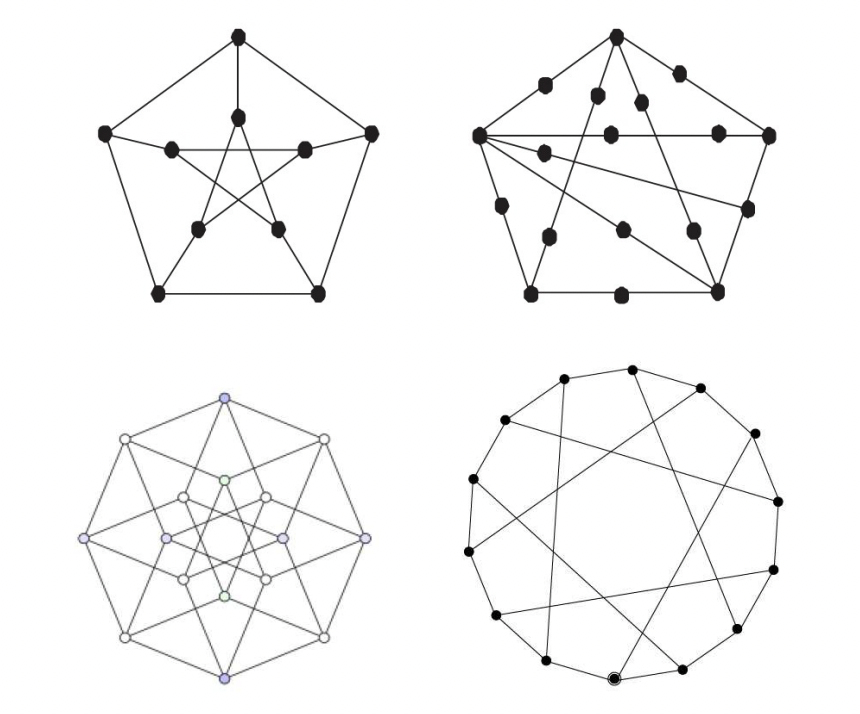
\includegraphics[width=.87\textwidth]{Q475}
\end{problem}

\begin{proof}[Solution]
    Since all four graphs have cycles, we can check by using the equation
    \[
        |E(G)| \leq \frac{g}{g - 2}(|V(G)| - 2),
    \]
    where $g$ is the length of the shortest cycle in the graph. 
    
    The graph on the top left has $15$ edges and $10$ vertices, and the shortest cycle has a length of $5$.
    \[
        15 > \frac{40}{3} = \frac{5}{5 - 2}(10 - 2),
    \]
    and thus it is not planar. 
    
    We can draw the graph on the top right in the following form:
    
    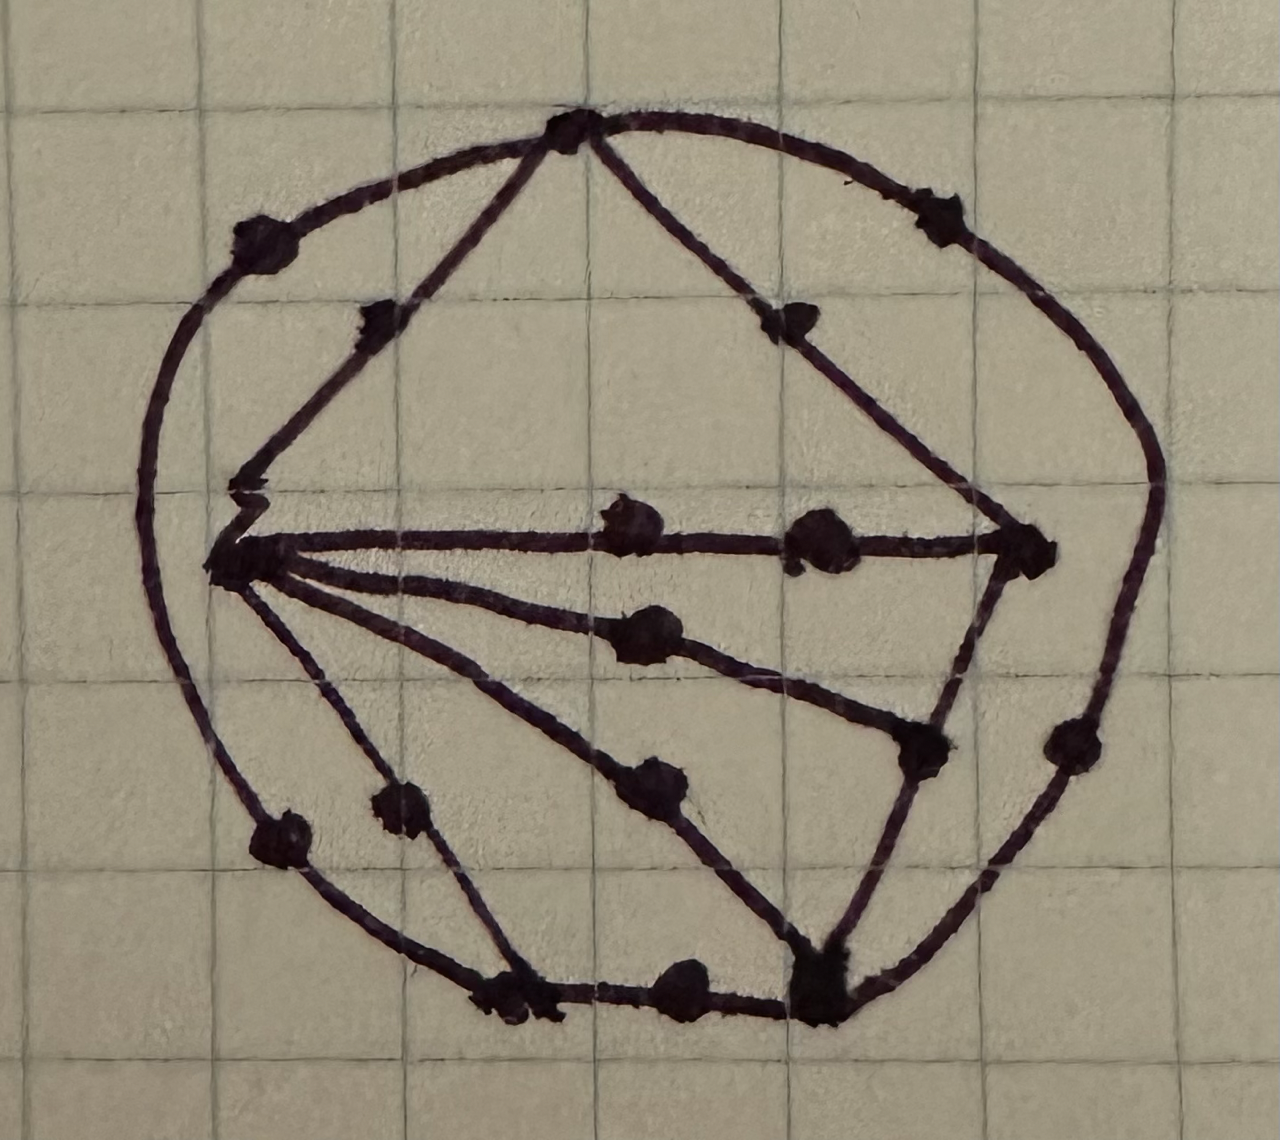
\includegraphics[width=.25\textwidth]{Q475-2} \\
    Therefore, the graph is planar.

    The graph on the bottom left has $32$ edges and $16$ vertices, and the shortest cycle has a length of $4$.
    \[
        32 > 28 = \frac{4}{4 - 2}(16 - 2),
    \]
    and thus it is not planar. 

    The graph on the bottom right has $20$ edges and $14$ vertices, and the shortest cycle has a length of $6$.
    \[
        20 > 18 = \frac{6}{6 - 2}(14 - 2),
    \]
    and thus it is not planar. 
\end{proof}

% 4.7.7
\begin{problem}{4.7.7}
    A maximal plane graph is a plane graph $G = (V, E)$ with $n \geq 3$ vertices such that if we join any two non-adjacent vertices in $G$, we obtain a non-plane graph
\end{problem}

\begin{enumerate}[label=(\alph*)]
    \item Draw a maximal plane graph on six vertices.

    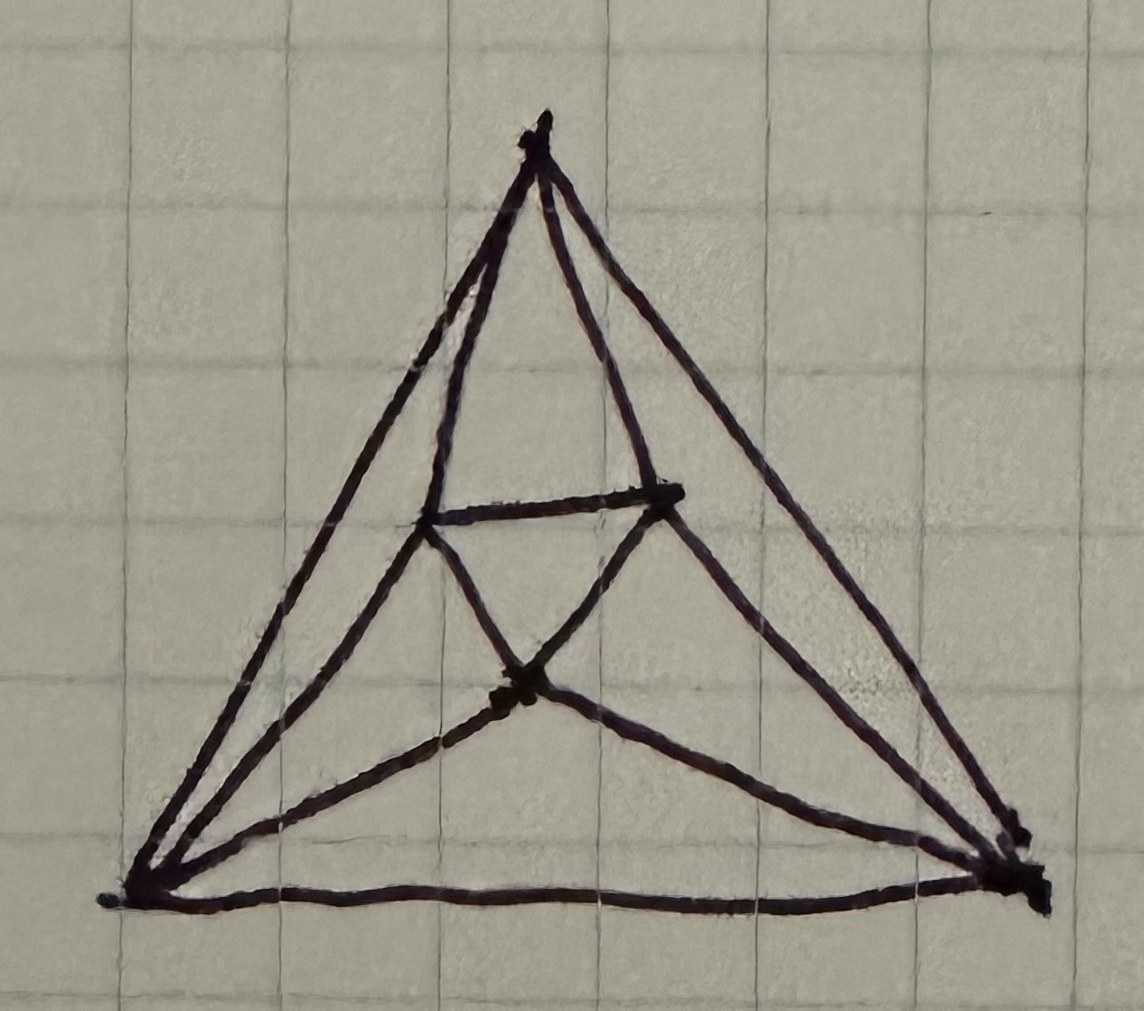
\includegraphics[width=.25\textwidth]{Q477a}

    \item Show that a maximal plane graph on $n$ points has $3n - 6$ edges and $2n - 4$ faces.

    \begin{proof}
        A maximal plane graph $G$ only contains triangular faces. $G$ is connected because if it's not, we can add an edge to connect two components and still get a plane graph, which contradicts $G$'s maximality. Let $n = |V(G)|$. By theorem, we know that $E(G) \leq 3n - 6$. Since $G$ is a maximal plane graph, we have $E(G) = 3n - 6$. By Euler's Formula, we have $n - (3n - 6) + |F(G)| = 2$. Therefore, rearranged, we have $|F(G)| = 2n - 4$ and $|E(G) = 3n - 6$.
    \end{proof}
    
    \item A triangulation of an $n$-gon is a plane graph whose vertex set is the vertex set of a convex $n$-gon in the plane, whose infinite face boundary is a convex $n$-gon, and all of whose other faces are triangles. How many edges does a triangulation of an $n$-gon have?
    
    \begin{proof}[Solution]
        To triangulate a $n$-gon, we can pick a vertex $v$ from the $n$-gon and connect it with all other vertices in the graph. Since $v$ is already connected to two vertices, we only need to add $n - 1 - 2 = n - 3$ edges. Therefore, including the original $n$ edges, a triangulation of an $n$-gon has $2n - 3$ edges.
    \end{proof}
\end{enumerate}

% 4.7.8
\begin{problem}{4.7.8}
    Show that every triangle-free planar graph is $4$-colorable.
\end{problem}

\begin{proof}
    Let $G$ be an $n$-vertex triangle-free planar graph. We will first check with Theorem $3$ in chapter $4$. Since the smallest possible cycle in $G$ is at least length $4$, we have 
    \[
        |E(G)| \leq 2(n - 2).
    \]
    Let $d$ be the sum of all degrees in $G$. By the Handshake Theorem, we know
    \[
        d = 2|E(G)| \leq 4n - 8.
    \]
    If $\delta(G) \geq 4$, then $d \geq 4n$, contradiction. Therefore, we can always find a vertex with a degree lesser or equal to $3$ in every triangle-free planar graph. We will then proceed by induction on $n$. We already know all paths are $4$-colorable. If $n = 4$, $G$ is a length $4$ cycle, which is $4$ colorable. Suppose $n > 4$. Pick a vertex $v$ from $G$ such that $d(v) \leq 3$. Since removing $v$ from $G$ does not create any triangles and the graph would remain planar, $G - \{v\}$ is $4$-colorable by induction. Since $v$ is connected to vertices of at most $3$ colors, we can assign the $4$th color to $v$. Therefore, every triangle-free planar graph is $4$-colorable.
\end{proof}

% 4.7.14
\begin{problem}{4.7.14}
    Let $\omega(G)$ – the clique number of $G$ – be the maximum number of vertices in a complete subgraph of a graph $G$.
\end{problem}

\begin{enumerate}[label=(\alph*)]
    \item Prove that for every graph $G$, $\chi(G) \geq \omega(G)$.

    \begin{proof}
        We know that $\chi(K_n) = n$. Since $K_{\omega(G)} \subseteq G$, we have $\chi(G) \geq \omega(G)$.
    \end{proof}

    \item Prove that for every graph $G$, $\chi(G) \geq |V(G)|/\alpha(G)$.

    \begin{proof}
        Suppose that we color $G$ with $\chi(G)$ colors. Let $C$ be a set of vertices with the same color. Since $e(C) = 0$, $C$ is an independent set. Thus, each set of vertices with the same color is an independent set and has a size less than $\alpha(G)$, and there are $\chi(G)$ of them. Therefore, $\alpha(G)\chi(G) \geq |V(G)|$, and, rearranged, we get $\chi(G) \geq |V(G)| / \alpha(G)$
    \end{proof}
    
    \item For each $k \geq 2$, find a graph $G$ such that $\chi(G) = k + 1$ and $\omega(G) = k$.
    
    \begin{proof}[Solution]
        For $k = 2$, a length $5$ cycle has $\omega(G) = k$ and $\chi(G) = k + 1$. For $k > 2$, we can start from a $k$-complete graph $F$ with a vertex set $\{s_1, s_2, \dots, s_k\}$, each colored differently with the set of colors $C = \{c_1, c_2, \dots, c_k\}$. Let $H = (V(F) \cup V, E(F) \cup E)$, where $V = \{b_1, b_2, \dots, b_k\}$ and $E = \{\{b_i, s_j\} : b_i \in V, \, s_j \in V(F), \, i \neq j\}$. Since each $b_i \in V(H)$ is connected to $k - 1$ vertices of different colors, there is still one color available for $b_i$, so we color $b_i$ with that color. Now all $b_i \in H$ are colored differently. We then add a vertex $v$ to $H$ and let $v$ form an edge with each $b_i \in V$, and we call this graph $G$. Since $v$ has $k$ neighbors with $k$ colors, it must be colored by a new color. Therefore, we get a graph $G$ where $\chi(G) = k + 1$ and $\omega(G) = k$. 
    \end{proof}

    Below is an illustration of what $G$ looks like when $k = 5$.

    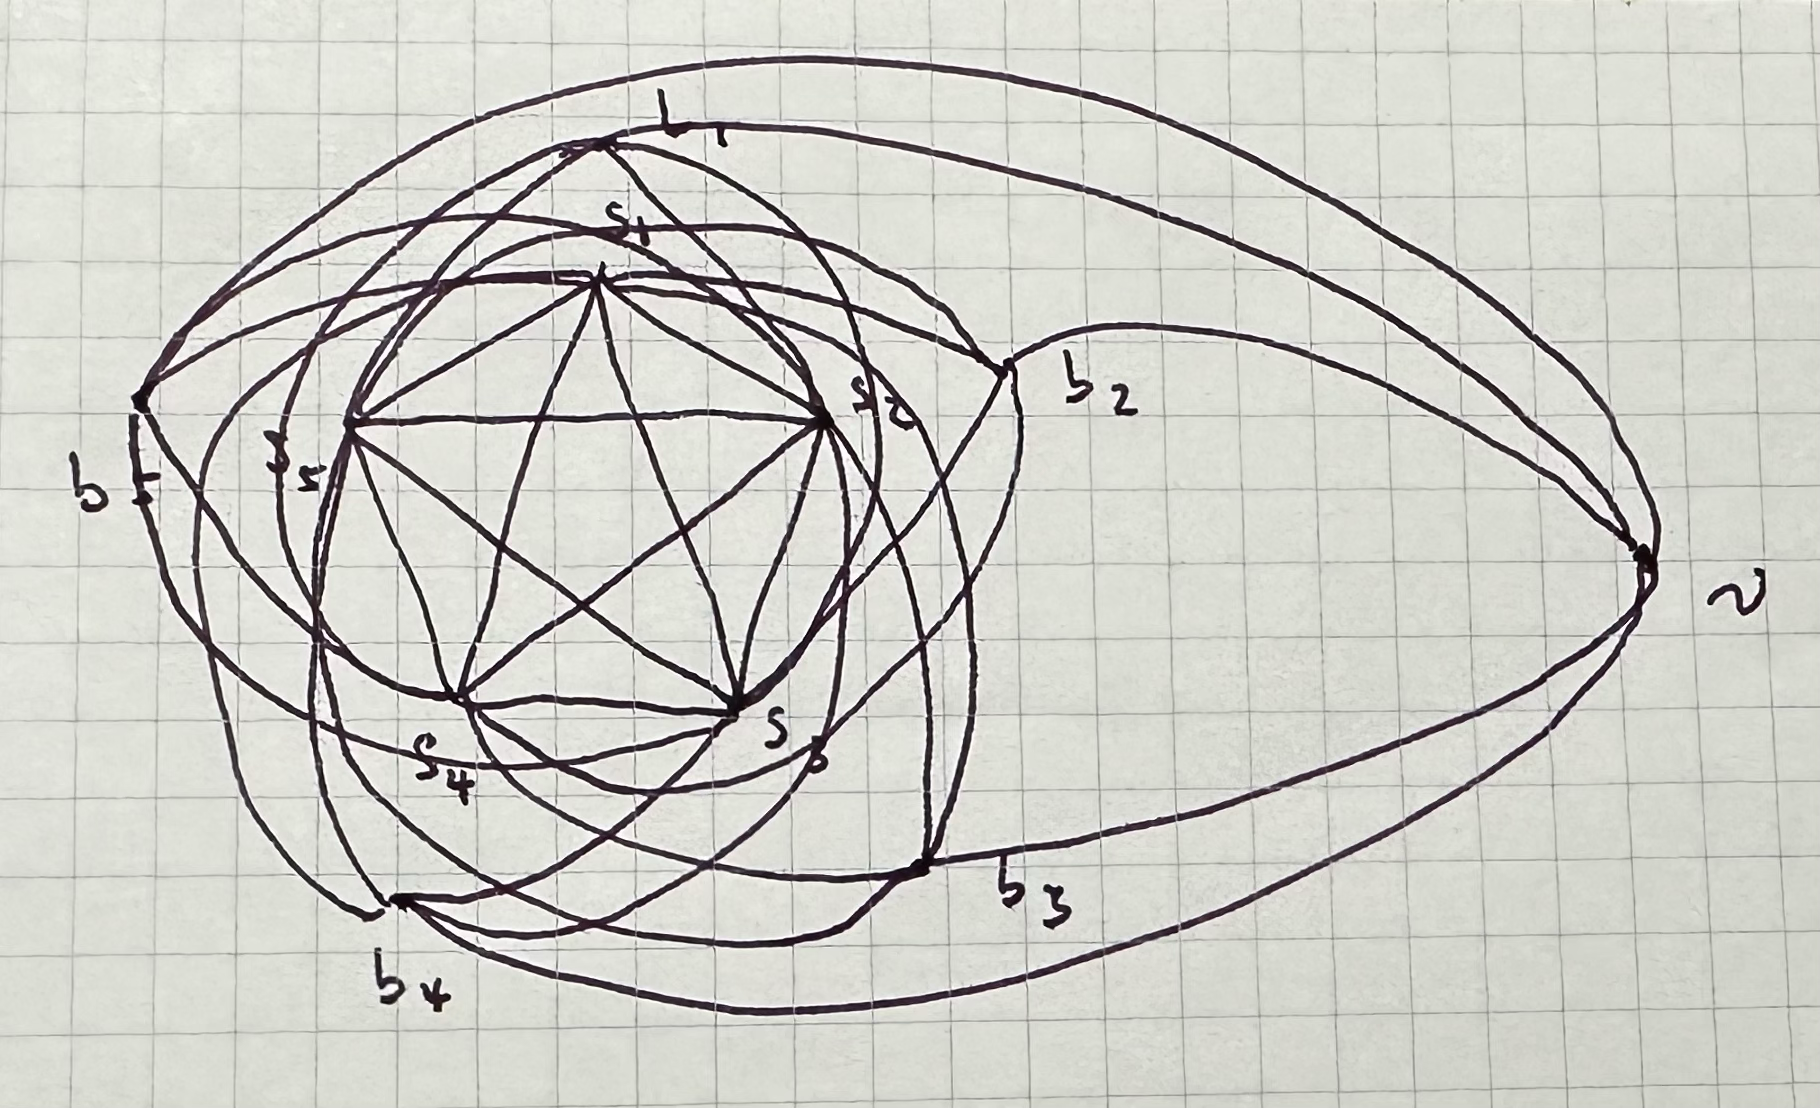
\includegraphics[width=.7\textwidth]{Q4714}
\end{enumerate}

% 5.9.2
\begin{problem}{5.9.2}
     Let $k \geq 1$. Prove that an $n$-vertex bipartite graph containing no matching of size $k$ has at most $(k - 1)(n - k + 1)$ edges for $n \geq 2k$. For each $k \geq 1$ and $n \geq 2k$, give an example of a graph with exactly $(k - 1)(n - k + 1)$ edges and no matching of size $k$.
\end{problem}

\begin{proof}
    Let $G$ be a $n$-vertex bipartite graph. For $n \geq 2k$, we prove by induction on $n$ that if $G$ has no matching of size $k$ and has at least $(k-1)(n - k + 1)$ edges, then $G = K_{k-1,n-k+1}$. For $n = 2k$, $G$ has at least $k^2 - 1$ edges. Suppose $G$ has parts with sizes $k + \gamma$ and $k - \gamma$, then $e(G) \leq (k + \gamma)(k - \gamma) = k^2 - \gamma^2$. Since $k^2 - \gamma^2 \geq e(G) \geq k^2 - 1$, $\gamma$ can only be $0$ or $1$. Suppose $\gamma = 0$. $G \neq K_{k,k}$ because it has no matching of size $k$. Suppose $G = K_{k,k} - \{u, v\}$, for some $u,v \in V(K_{k,k})$. Since $G$ contains a $K_{k-1,k-1}$ that does not contain $v$ and some vertex $w \neq u$, $G$ has a matching $M$ of size $k - 1$ such that $\{u, w\} \notin M$. Since $u,w$ forms an edge in $G$, $M \cup \{u, w\}$ is a matching of $G$ with size $k$. Thus, for $n = 2k$, $G = K_{k-1,k+1}$. 
    
    For $n \geq 2k + 1$, let $G$ be an $n$-vertex graph with no matching of size $k$ and $e(G) \geq (k-1)(n - k + 1)$. Let $H$ be a subgraph with $(k-1)(n - k + 1)$ edges. Suppose for the sake of contradiction that $\delta(H) \geq k$. Let $P$ be the longest path in $H$, say $v_1v_2\dots v_m$. We know $N(v_1) \subseteq V(P)$. Since $H$ is bipartite, $H$ does not contain any triangles, so there exists $v_i \in N(v_1)$ for some $2k \leq i \leq m$. Thus, $v_1v_2\cdots v_iv_1$ is a cycle of length at least $2k$ in $H$, and the cycle contains a matching of size $k$, contradiction. Thus, $\delta(H) \leq k - 1 = \delta(K_{k-1,n-k+1})$. If $v$ is a vertex of minimum degree in $H$, then 
    \begin{align}
        e(H - \{v\}) 
        &\geq e(K_{k-1,n-k+1}) - \delta(K_{k-1,n-k+1}) \\
        &= (k-1)(n-k+1) - (k-1) = e(K_{k-1,n-k}).
    \end{align}
    By induction, $H - \{v\} = K_{k-1,n-k}$, and so $d_H(v) = (k-1)(n - k + 1) - e(K_{k-1,n-k}) = k - 1$. Let $A,B$ be parts of $H - \{v\}$ such that $|A| = k - 1$ and $|B| = n - k$. Suppose for sake of contradiction that $A \cup \{v\}$ is a part of $H$. Let $S \subset A \cup \{v\}$ such that $S \neq \emptyset$. If $S = \{v\}$, then $|N(S)| = k - 1 \geq |S|$. If $S \neq \{v\}$, then $S \cap A \neq \emptyset$. Since each vertex in $A$ is connected to all vertices in $B$, $|N(S)| = |B| = n - k \geq |S|$. By Hall's Theorem, there is a matching saturating $A \cup \{v\}$, which has a size of $k$, contradiction. Therefore, $B \cup \{v\}$ is part of $H$, so $H = K_{k-1,n-k+1}$. Since $K_{k-1,n-k+1}$ is a maximal graph that has no matching of size $k$, $G = H = K_{k-1,n-k+1}$, and thus $G$ is an example of the required graph.
\end{proof}

% 5.9.3
\begin{problem}{5.9.3}
     Determine for all $n \geq 1$ the value of ex$(n, P_3)$.
\end{problem}

\begin{proof}
    By the Erdös-Gallai Theorem, we know ex$(n, P_3) \leq n$, with equality if and only if $3|n$ and every component of the graph is $K_3$. Thus, if $3|n$, a graph that consists of a union of $K_3$ has $n$ edges and is a maximal graph that does not contain any $P_3$, so ex$(n, P_3) \geq n$. If $3 \nmid n$, we have ex$(n, P_3) \leq n - 1$. Since $K_{n-1,1}$ is a maximal graph that has no $P_3$ and $e(K_{n-1,1}) = n - 1$, ex$(n, P_3) \geq n - 1$. Therefore, \[
        \text{ex}(n,P_3)= \begin{cases}
        n,      & \text{if } n | 3 \\
        n - 1,  & \text{otherwise}.
        \end{cases}
    \]
\end{proof}

\begin{problem}{5.9.8}
    Let $G$ be a graph. Prove that there exists a partition $(A, B)$ of $V(G)$ such that $e(A,B) \geq \frac{1}{2}e(G)$ and $|A| \leq |B| \leq |A| + 1$.
\end{problem}

\begin{proof}
    We will first prove by induction on $n$ to show that there exists a partition $(A, B)$ of $V(G)$ such that $e(A,B) \geq \frac{1}{2}e(G)$ and $|A| = |B|$, for $n = |V(G)|$ is even. The case $n = 2$ is true since $e(A, B) = e(G)$. For $n > 2$, we remove two vertices $u, v$ from $G$ and obtain $G'$. By induction, there exists a partition $(A', B')$ of $V(G')$ such that $e(A', B') \geq \frac{1}{2}(e(G) - d(u) - d(v))$ and $|A'| = |B'|$. Since $d(u) + d(v) = e(u, A') + e(u, B') + e(v, A') + e(u, B')$, we know $\max(e(u, A') + e(v, B'), e(u, B') + e(v, A')) \geq \frac{1}{2}(d(u) + d(v))$. Suppose without loss of generality that $e(u, A') + e(v, B') \geq \frac{1}{2}(d(u) + d(v))$. Let $A = A' \cup \{v\}$, $B = B' \cup \{u\}$. Then $(A, B)$ is a partition of $V(G)$ such that $e(A, B) \geq \frac{1}{2}e(G)$. 
    
    Suppose that $n$ is odd. Let $v \in G$. We know there exists a partition $(A',B')$ of $V(G)\backslash \{v\}$ such that $e(A',B') \geq \frac{1}{2}(e(G) - d(v))$ and $|A'| = |B'|$. Since $d(v) = e(v, A') + e(v, B')$, $\max(e(v, A'), e(v, B')) \geq \frac{1}{2}d(v)$. Suppose, without loss of generality, that $e(v, A') \geq \frac{1}{2}d(v)$. Let $A = A'$, $B = B' \cup \{v\}$. Then $(A,B)$ is a partition of $V(G)$ such that $e(A,B) \geq \frac{1}{2}e(G)$.
\end{proof} 

\begin{problem}{5.9.10}
    A bowtie is a graph $B$ consisting of two triangles sharing exactly one vertex. Determine $\text{ex}(n, B)$ for all $n \geq 1$.
\end{problem}
\begin{proof}
    Let $G$ be a graph with at least $\left\lfloor\frac{n^2}{4}\right\rfloor + 1$ egdes. $G$ does not contain $B$ for $n < 5$, so we can assume $n \geq 5$. We will prove by induction on $n$ to show that if $G$ does not contain $B$ then $G$ is a balanced complete bipartite graph plus an edge. If $n = 5$
\end{proof}

\begin{problem}{5.9.12}
    Let $G$ be a bipartite graph with parts of sizes $m$ and $n$, not containing a $4$-cycle. Prove that
    \[
        |E(G)| \leq m\sqrt{n} + m + n
    \]
\end{problem}

\begin{proof}
    Let $M, N$ be parts of $G$ such that $|M| = m$, $|N| = n$. We count the number of $K_{1,2}$. Since no set of $2$ vertices have more than $1$ common neighbor, we get
    \[
        \sum_{v \in N} { d(v) \choose 2 } \leq { m \choose 2 } \leq \frac{m^2}{2}.
    \]
    Let $d$ be the average degree of the vertices in $N$. If $d \leq 1$, then we are done as $|E(G)| = nd \leq n$. Suppose $d \geq 2$. Define $f : \mathbb{R} \rightarrow \mathbb{R}$ to be $f(x) = \begin{cases}
        { x \choose 2 } &, x \geq 2 \\
        0 &, x < 2
    \end{cases}$. Since $f$ is convex, Jensen's inequality gives 
    \[
        \sum_{v \in N} { d(v) \choose 2 } \geq n{ d \choose 2 } \geq \frac{n(d - 1)^2}{2}.
    \]
    Thus, we get 
    \begin{gather}
        n(d - 1)^2 \leq m^2 \\
        d \leq \frac{m}{\sqrt{n}} + 1
    \end{gather}
    Therefore, $|E(G)| = nd \leq m\sqrt{n} + n \leq m\sqrt{n} + m + n$.
\end{proof}

\begin{problem}{6.3.9}
    Prove that for $n > 2^k$, every k-coloring of $E(K_n)$ gives a monochromatic odd cycle
\end{problem}

\begin{proof}
    Suppose for sake of contradiction that $G$ is a $k$-edge-colored $K_n$ with no monochromatic odd cycle, for $n \geq 2^k + 1$. $G$ contains a subgraph $k$-colored $K_{2^k+1}$ with no monochromatic odd cycle, we name it $G_k$. We obtain $H \subseteq G_k$ by picking a color from $G_k$ and removing all edges that are not that color. Since $G_k$ contains no monochromatic odd cycles, $H$ is bipartite, say with parts $A$, $B$. Assume, without loss of generality, that $|A| \geq 2^{k-1} + 1$. Let $H' = G[A]$. Then $H'$ contains a $(k-1)$-edge-coloring of a $K_{2^{k-1} + 1}$ with no monochromatic odd cycle, we name it $G_{k-1}$. By recursively finding a smaller $G_r$, we can find $G_3$, a $1$-edge-colored $K_3$ with no monochromatic odd cycle, contradiction. Therefore, $G$ contains a monochromatic odd cycle.
\end{proof}

% \begin{problem}{6.?.?}
%     It is known that if an $n$-vertex graph $G$ is triangle-free and has a maximum degree $d \geq 1$, then $G$ contains an independent set of size at least $n(\log{d})/2d$. Prove that for $t \geq 3$,
%     \[
%         r(3,t) \leq \frac{2t^2}{\log{t}}.
%     \]
% \end{problem}

% \begin{proof}
%     Let $n \geq \frac{2t^2}{\log{t}}$ and let $G = K_n$. We will show that any two coloring of $E(G)$ contain a red $K_3$ or a blue $K_t$. Let $R$, $B$ each be the graph of edges of the color red and blue respectively. Suppose $R$ is triangle-free and there exists $v \in V(R)$ with $d_R(v) \geq t$. Since $\Delta(R) \geq t$, by the given fact, we know $R$ contains an independent set $I$ of size of at least $n(\log{t})/2t = t$, which means that $I$ forms a blue $K_t$ in $G$, contradiction. Thus, we can assume $\Delta(R) \leq t -1$, and so $\delta(B) \geq n - t$. Since $\frac{n}{2} \geq \frac{t^2}{\log{t}} \geq t$ for $t \geq 3$, $\delta(B) \geq \frac{n}{2}$. Suppose $B$ is $K_t$ free. Then by Turan's Theorem, $\delta(B) \leq \delta(T_{t - 1}(n)) \leq n - \left\lceil\frac{n}{t - 1}\right\rceil \leq n - \frac{n}{t - 1}$. Thus, we then have 
% \end{proof}

\end{document}